
\documentclass{standalone}
\usepackage[utf8]{inputenc}
\usepackage{pgfplots}
\pgfplotsset{compat=newest}

\usepgfplotslibrary{groupplots}
\definecolor{printable_1}{RGB}{137, 197, 64}
\definecolor{printable_2}{RGB}{247, 124, 0}
\definecolor{printable_3}{RGB}{ 17, 148, 246}
\definecolor{printable_4}{RGB}{103, 52, 186}

\usetikzlibrary{external}
\usepackage{calc}


\begin{document}
    \begin{tikzpicture}
	    	\node (is) at (-9, 0.35) {Input Space $\mathcal{I}$};
	    	\node (fs) at (-9, -0.92) {Feature Space  $\mathcal{F}$};
	    	\node  (c) at (-9, -2.25) {Classifier  $c(\cdot)$};
    
    		\draw[-stealth] (is.south) -- (fs.north);
    		\draw[-stealth] (fs.south) -- (c.north);

    		%\draw (-8, -2.25) -- (10, -2.25);
    
	        \node[inner sep=0pt] (ts) at (0,0)
	        {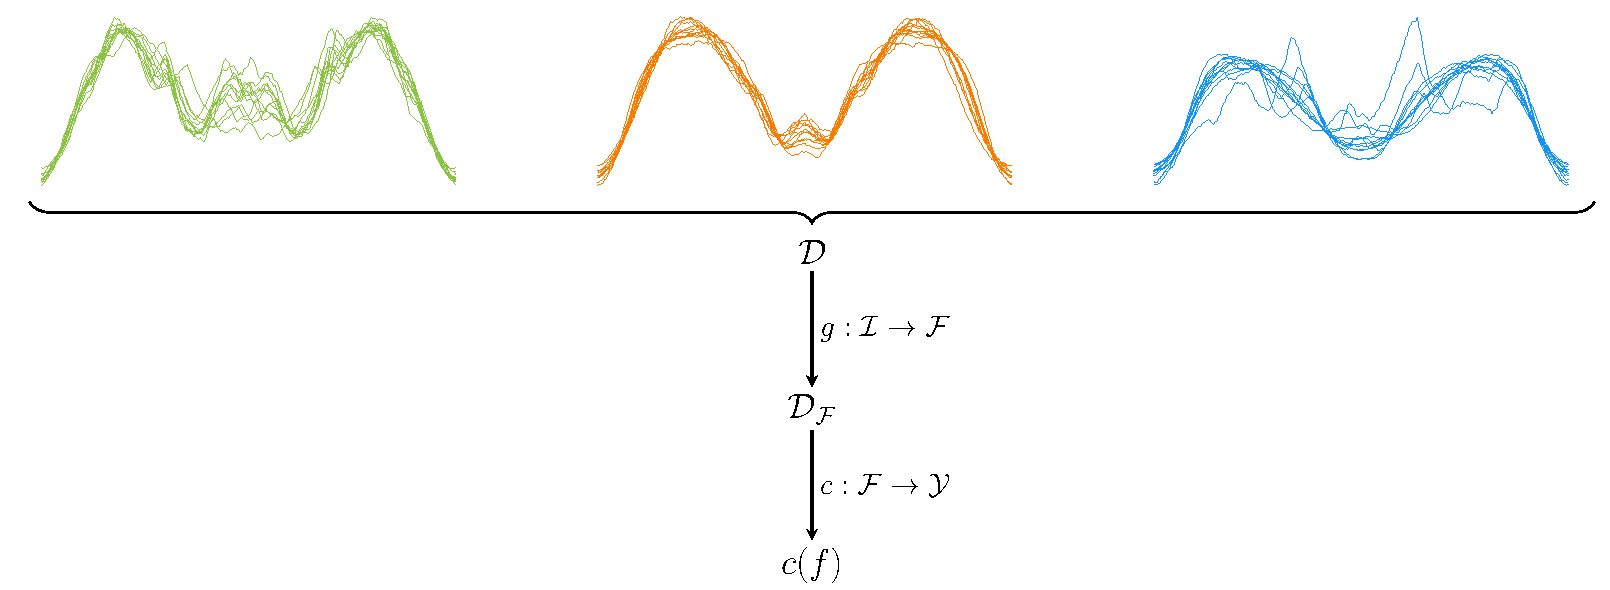
\includegraphics[width=1.1\textwidth]{timeseries.pdf}};
	        
	        \node[inner sep=0pt] (hist) at (0.07,-4.7)
	        {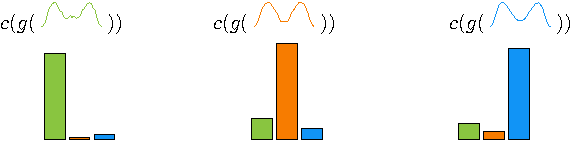
\includegraphics[width=.8\textwidth]{histograms.pdf}};
			
			\draw[-stealth, thick] ($(ts.south)+ (0.07, 0)$) -- node {} +(0, -0.8);				
			\draw[-stealth, thick] ($(ts.south)+ (0.07, 0)$) -- node {} +(-2.6, -0.8);
			\draw[-stealth, thick] ($(ts.south)+ (0.07, 0)$) -- node {} +(2.6, -0.8);
			
    \end{tikzpicture}
\end{document}